\documentclass[12pt]{article} 
\usepackage{pythonhighlight}

\usepackage[utf8]{inputenc}

% font types
\renewcommand{\familydefault}{\sfdefault}
% \usepackage{helvet}
% \usepackage[T1]{fontenc}
% \usepackage[utf8]{inputenc}

% package to rotate the page landscape 
%\usepackage[paper=portrait, pagesize]{typearea}
\usepackage[a4paper]{geometry}
\usepackage[usegeometry]{typearea}
%\usepackage[hmargin=.65in,vmargin=1.1in]{geometry}
%\usepackage[top=0.75in, left=0.75in, right=0.52in, bottom=1.44in]{geometry}

% only for dummy text
\usepackage{blindtext}
\usepackage{lipsum}
%\usepackage[margin=0.5in, left=0.5in, top=0.8in, includefoot]{geometry}
%\usepackage[a4paper, left=1.0in, right=1.0in, top=1.0in, bottom=1.0in]{geometry}

\usepackage[hidelinks]{hyperref} % Allows for clickable references

% Graphics preamble
\usepackage{graphicx} % import graphics package
%\graphicspath{ {/Users/tgol0003/Desktop/seagate4_2/uwgeo_models/production_models/} } % harddisk path
\usepackage{float} % Allows for control of float positions
\usepackage[section]{placeins} % to place figures in the section 
\usepackage{multicol} % position figures across the columns

% figures packages

% adding number with in section to equations
\usepackage{amsmath} 
\numberwithin{equation}{subsection} 
\makeatletter
\@addtoreset{equation}{section}
\makeatother

% Header and Footer info
\usepackage{fancyhdr}
\pagestyle{fancy}
\fancyhead{}
\fancyfoot{}
\fancyfoot[R]{\thepage}
\renewcommand{\headrulewidth}{0pt}
\renewcommand{\footrulewidth}{0pt}

\usepackage{changepage}

\newgeometry{left=0.35in, right=0.35in, top=0.5in, bottom=1.0in}


\begin{document} 

\cleardoublepage
\KOMAoptions{paper=portrait}
\recalctypearea
\newgeometry{left=0.1in, right=0.1in, top=0.1in, bottom=0.1in}

% \eject \pdfpagewidth=3in \pdfpageheight=10in % command to change the page height and width
\eject \pdfpagewidth=11.4in \pdfpageheight=10.8in 

\newpage

\vspace{1.5in} 

\begin{adjustwidth}{10cm}{1cm}
	\vspace{5.5in}  
	\textbf{Annulus Benchmark: Thieulot\&Puckett 2018}
\end{adjustwidth}

\newpage

\textbf{Benchmark Case}
\vspace{0.2in}

\begin{adjustwidth}{1cm}{5cm}
	\hspace{0.2in} This benchmark creates an isoviscous, isothermal solution of the incompressible Stokes
	equations for which simple kinematic boundary conditions lead to structures that are 
	serve as a model of "convection cells", where the number of these cells is determined
	by a single parameter k. In this case, the velocity is only prescribed on the inner and 
	outer boundaries  $r = R_{1}, R_{2}$ and in what follows we have set $\rho_{0} = 0$.
\end{adjustwidth}

\vspace{0.2in}

\begin{adjustwidth}{1cm}{5cm}
	\begin{python}
		# boundary conditions
		v_diff =  v_uw.sym - v_ana.sym
		stokes.add_natural_bc(2.5e6*v_diff, "Upper")
		stokes.add_natural_bc(2.5e6*v_diff, "Lower")
	\end{python}
\end{adjustwidth}


%\vspace{1.2in}
%\textbf{Mesh}
%\begin{figure*}[!htb]
%	
%	\begin{multicols}{4}
%		\includegraphics[width=7cm]{./modelT_p_res_5_k_0/mesh.png}\par
%		\hspace{0.75in}
%		\includegraphics[width=7cm]{./modelT_p_res_5_k_1/mesh.png}\par
%		\hspace{1.5in}
%		\includegraphics[width=7cm]{./modelT_p_res_5_k_2/mesh.png}\par
%		\hspace{2.25in}
%		\includegraphics[width=7cm]{./modelT_p_res_5_k_4/mesh.png}
%	\end{multicols}
%	
%\end{figure*}

%\newpage
%\textbf{Density, Velocity, Pressure}
%\begin{figure*}[!htb]
%	
%	\begin{multicols}{4}
%		\includegraphics[width=7cm]{./modelT_p_res_5_k_0/rho_ana.png}\par
%		\hspace{0.75in}
%		\includegraphics[width=7cm]{./modelT_p_res_5_k_1/rho_ana.png}\par
%		\hspace{1.5in}
%		\includegraphics[width=7cm]{./modelT_p_res_5_k_2/rho_ana.png}\par
%		\hspace{2.25in}
%		\includegraphics[width=7cm]{./modelT_p_res_5_k_4/rho_ana.png}
%	\end{multicols}
%	\vspace{-0.3in}
%	\begin{multicols}{1}
%		\hspace{4.0in} 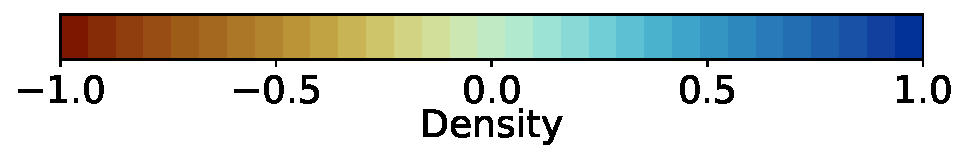
\includegraphics[width=8cm]{./modelT_p_res_5_k_0/rho_ana_cbhorz.pdf}
%	\end{multicols}
%	
%	\vspace{-0.3in}
%	
%	\begin{multicols}{4}
%		\includegraphics[width=7cm]{./modelT_p_res_5_k_0/vel_uw.png}\par
%		\hspace{0.75in}
%		\includegraphics[width=7cm]{./modelT_p_res_5_k_1/vel_uw.png}\par
%		\hspace{1.5in}
%		\includegraphics[width=7cm]{./modelT_p_res_5_k_2/vel_uw.png}\par
%		\hspace{2.25in}
%		\includegraphics[width=7cm]{./modelT_p_res_5_k_4/vel_uw.png}
%	\end{multicols}
%	\vspace{-0.3in}
%	\begin{multicols}{1}
%		\hspace{4.0in} 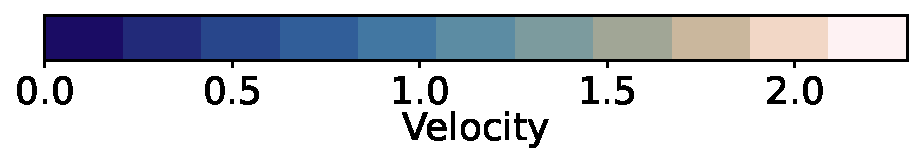
\includegraphics[width=8cm]{./modelT_p_res_5_k_0/v_ana_cbhorz.pdf}
%	\end{multicols}
%	
%	\vspace{-0.3in}
%	\begin{multicols}{4}
%		\includegraphics[width=7cm]{./modelT_p_res_5_k_0/p_uw.png}\par
%		\hspace{0.75in}
%		\includegraphics[width=7cm]{./modelT_p_res_5_k_1/p_uw.png}\par
%		\hspace{1.5in}
%		\includegraphics[width=7cm]{./modelT_p_res_5_k_2/p_uw.png}\par
%		\hspace{2.25in}
%		\includegraphics[width=7cm]{./modelT_p_res_5_k_4/p_uw.png}
%	\end{multicols}
%	\vspace{-0.3in}
%	\begin{multicols}{1}
%		\hspace{4.0in} 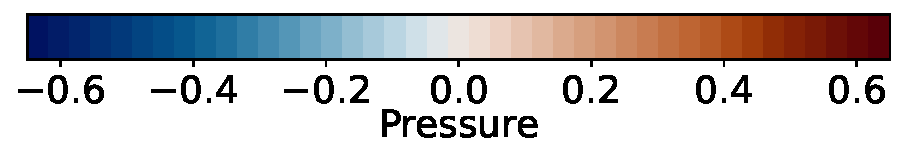
\includegraphics[width=8cm]{./modelT_p_res_5_k_0/p_ana_cbhorz.pdf}
%	\end{multicols}
%	
%\end{figure*}

\newpage
\textbf{$L_{2}$ norm of the error}

\begin{adjustwidth}{1cm}{5cm}
	Velocity penalty: 2.5e6 (magenta), 1e8 (green), 1e10 (skyblue) \newline
	Stokes tolerance: 1e-10 \newline
	Stokes element: $P_{2}P_{1}$
\end{adjustwidth}


\begin{figure*}[!htb]
		\begin{multicols}{1}
				\hspace{3.0in} 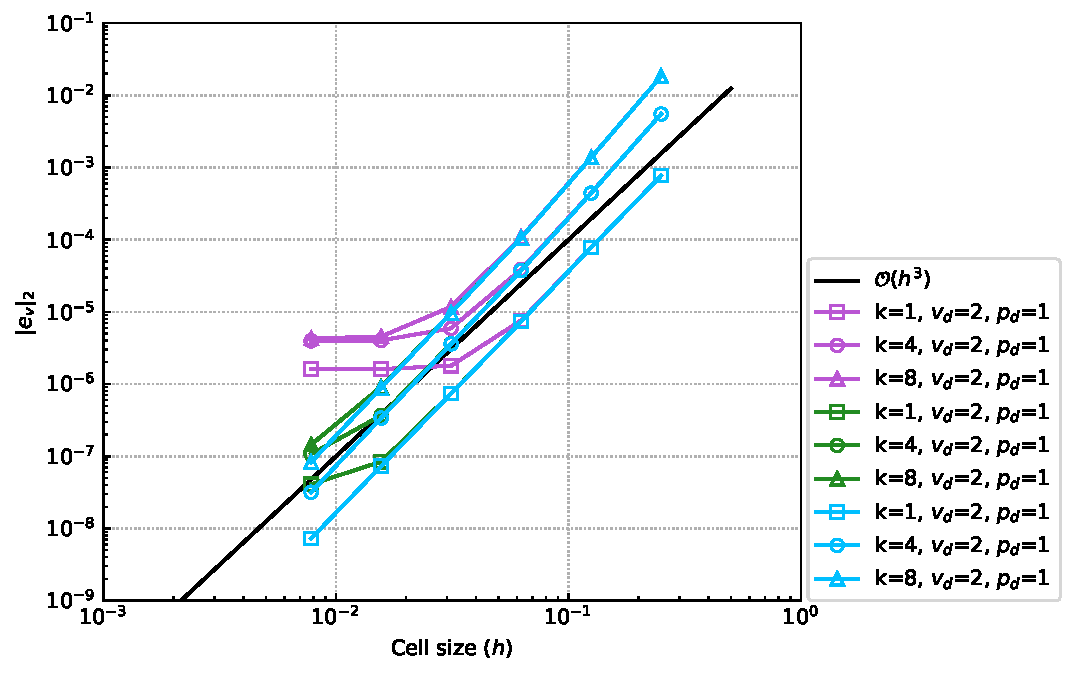
\includegraphics[width=17cm]{../Annulus_Benchmark_Thieulot/benchmark_figs/vel_err_conv_vel_penalty_1.0e+10_stokes_tol_1.0e-10_all_v_pen.pdf}
		\end{multicols}
		
		\begin{multicols}{1}
			\hspace{3.0in} 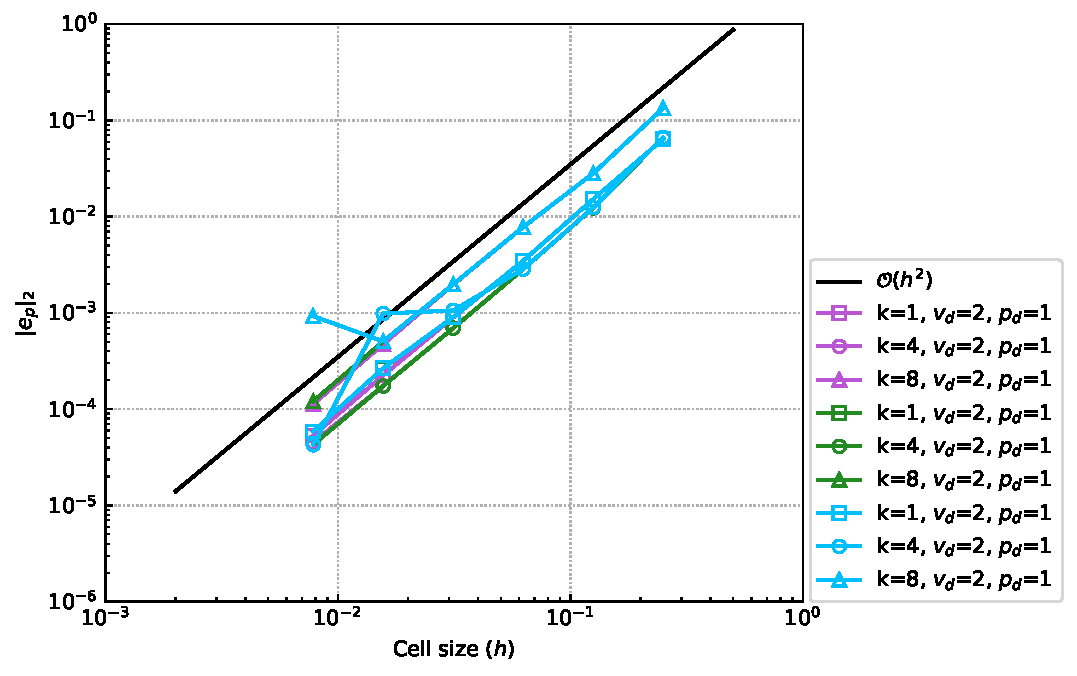
\includegraphics[width=17cm]{../Annulus_Benchmark_Thieulot/benchmark_figs/p_err_conv_vel_penalty_1.0e+10_stokes_tol_1.0e-10_all_v_pen.pdf}
		\end{multicols}
\end{figure*}

\newpage
\textbf{$L_{2}$ norm of the error}

\begin{adjustwidth}{1cm}{5cm}
	Stokes elements: $P_{1}P_{0} (disc. pressure), P_{2}P_{1}, P_{3}P_{2}$  \newline
	Velocity penalty: 2.5e6, 1e10, 1e10 \newline
	Stokes tolerance: 1e-7, 1e-10, 1e-10
\end{adjustwidth}


\begin{figure*}[!htb]
	\begin{multicols}{1}
		\hspace{3.0in} 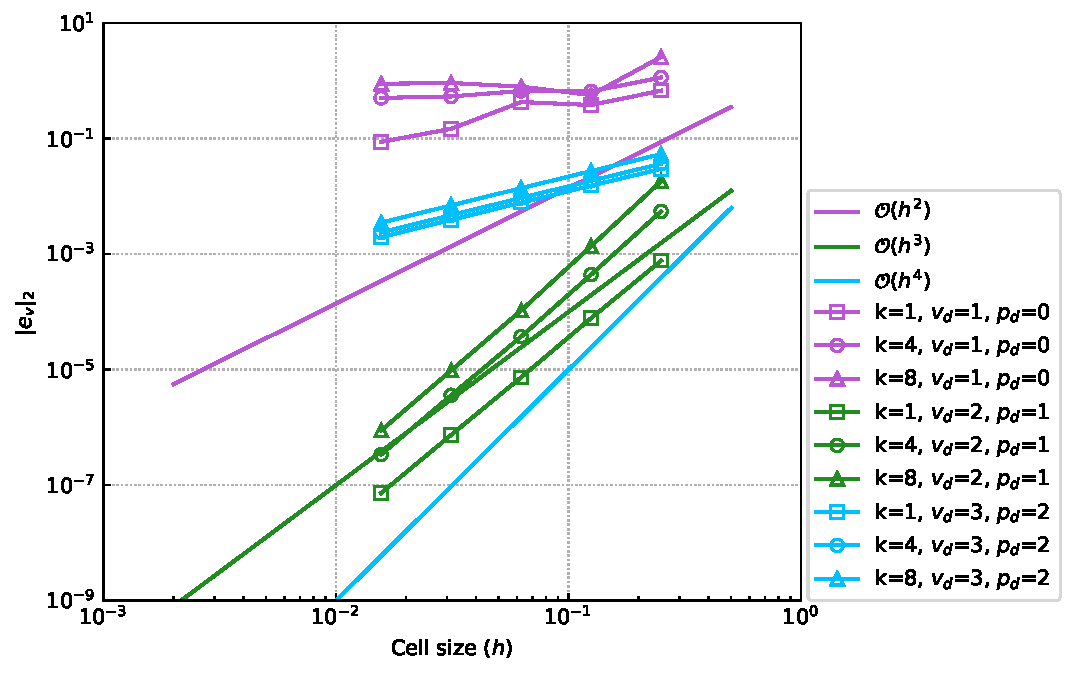
\includegraphics[width=17cm]{../Annulus_Benchmark_Thieulot/benchmark_figs/vel_err_conv_vel_penalty_1.0e+10_stokes_tol_1.0e-10_all_k.pdf}
	\end{multicols}
	
	\begin{multicols}{1}
		\hspace{3.0in} 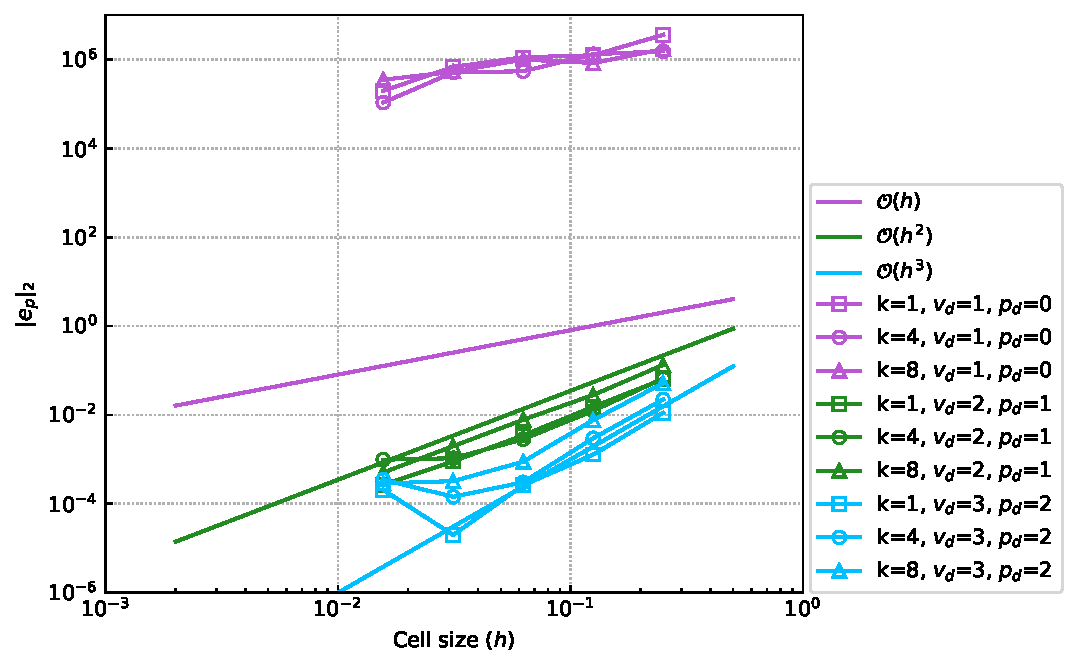
\includegraphics[width=17cm]{../Annulus_Benchmark_Thieulot/benchmark_figs/p_err_conv_vel_penalty_1.0e+10_stokes_tol_1.0e-10_all_k.pdf}
	\end{multicols}
\end{figure*}

\end{document}